\graphicspath{{images/mechanics}}

\section{Mechanik}

In der Nächsten Sektion wird die Mechanik der Fotobox beschrieben.
Die Mechanik ist ein sehr wichtiger Teil der Fotobox, da sie das erste
ist, was der Endbenutzer sieht. Sie sollte daher ansprechend und so stabil
aufgebaut sein, dass sie auch bei häufigem Transport nicht beschädigt wird.
Daher werde ich nun erläutern, warum ich mich für das aktuelle Design entschieden habe
und welche Probleme ich dabei hatte.

\begin{figure}[H]
    \centering
    
\includegraphics[width=1\textwidth]{fotobox_frontplatte_v2.png}
    \caption{Die erste Version der Frontplatte.}
    \label{fig:frontplatte_v1}
\end{figure}

In der Abbildung \ref{fig:frontplatte_v1} ist die erste Version der Frontplatte zu sehen.
In den löchern eins und zwei sollten jeweils ein Blitz und eine LED Lampe platziert werden,
in dem mittleren Loch mit der Nummer drei sollte die Kamera platziert werden.


Jedoch hat sich herausgestellt, dass durch die seitliche Platzierung des Blitzes
das Motiv einen seitlichen Schatten wirft. Was die Qualität der Bilder deutlich verringert,
da das Bild auch nicht einheitlich ausgeleuchtet wird.

\newpage
\begin{figure}[H]
    \centering
    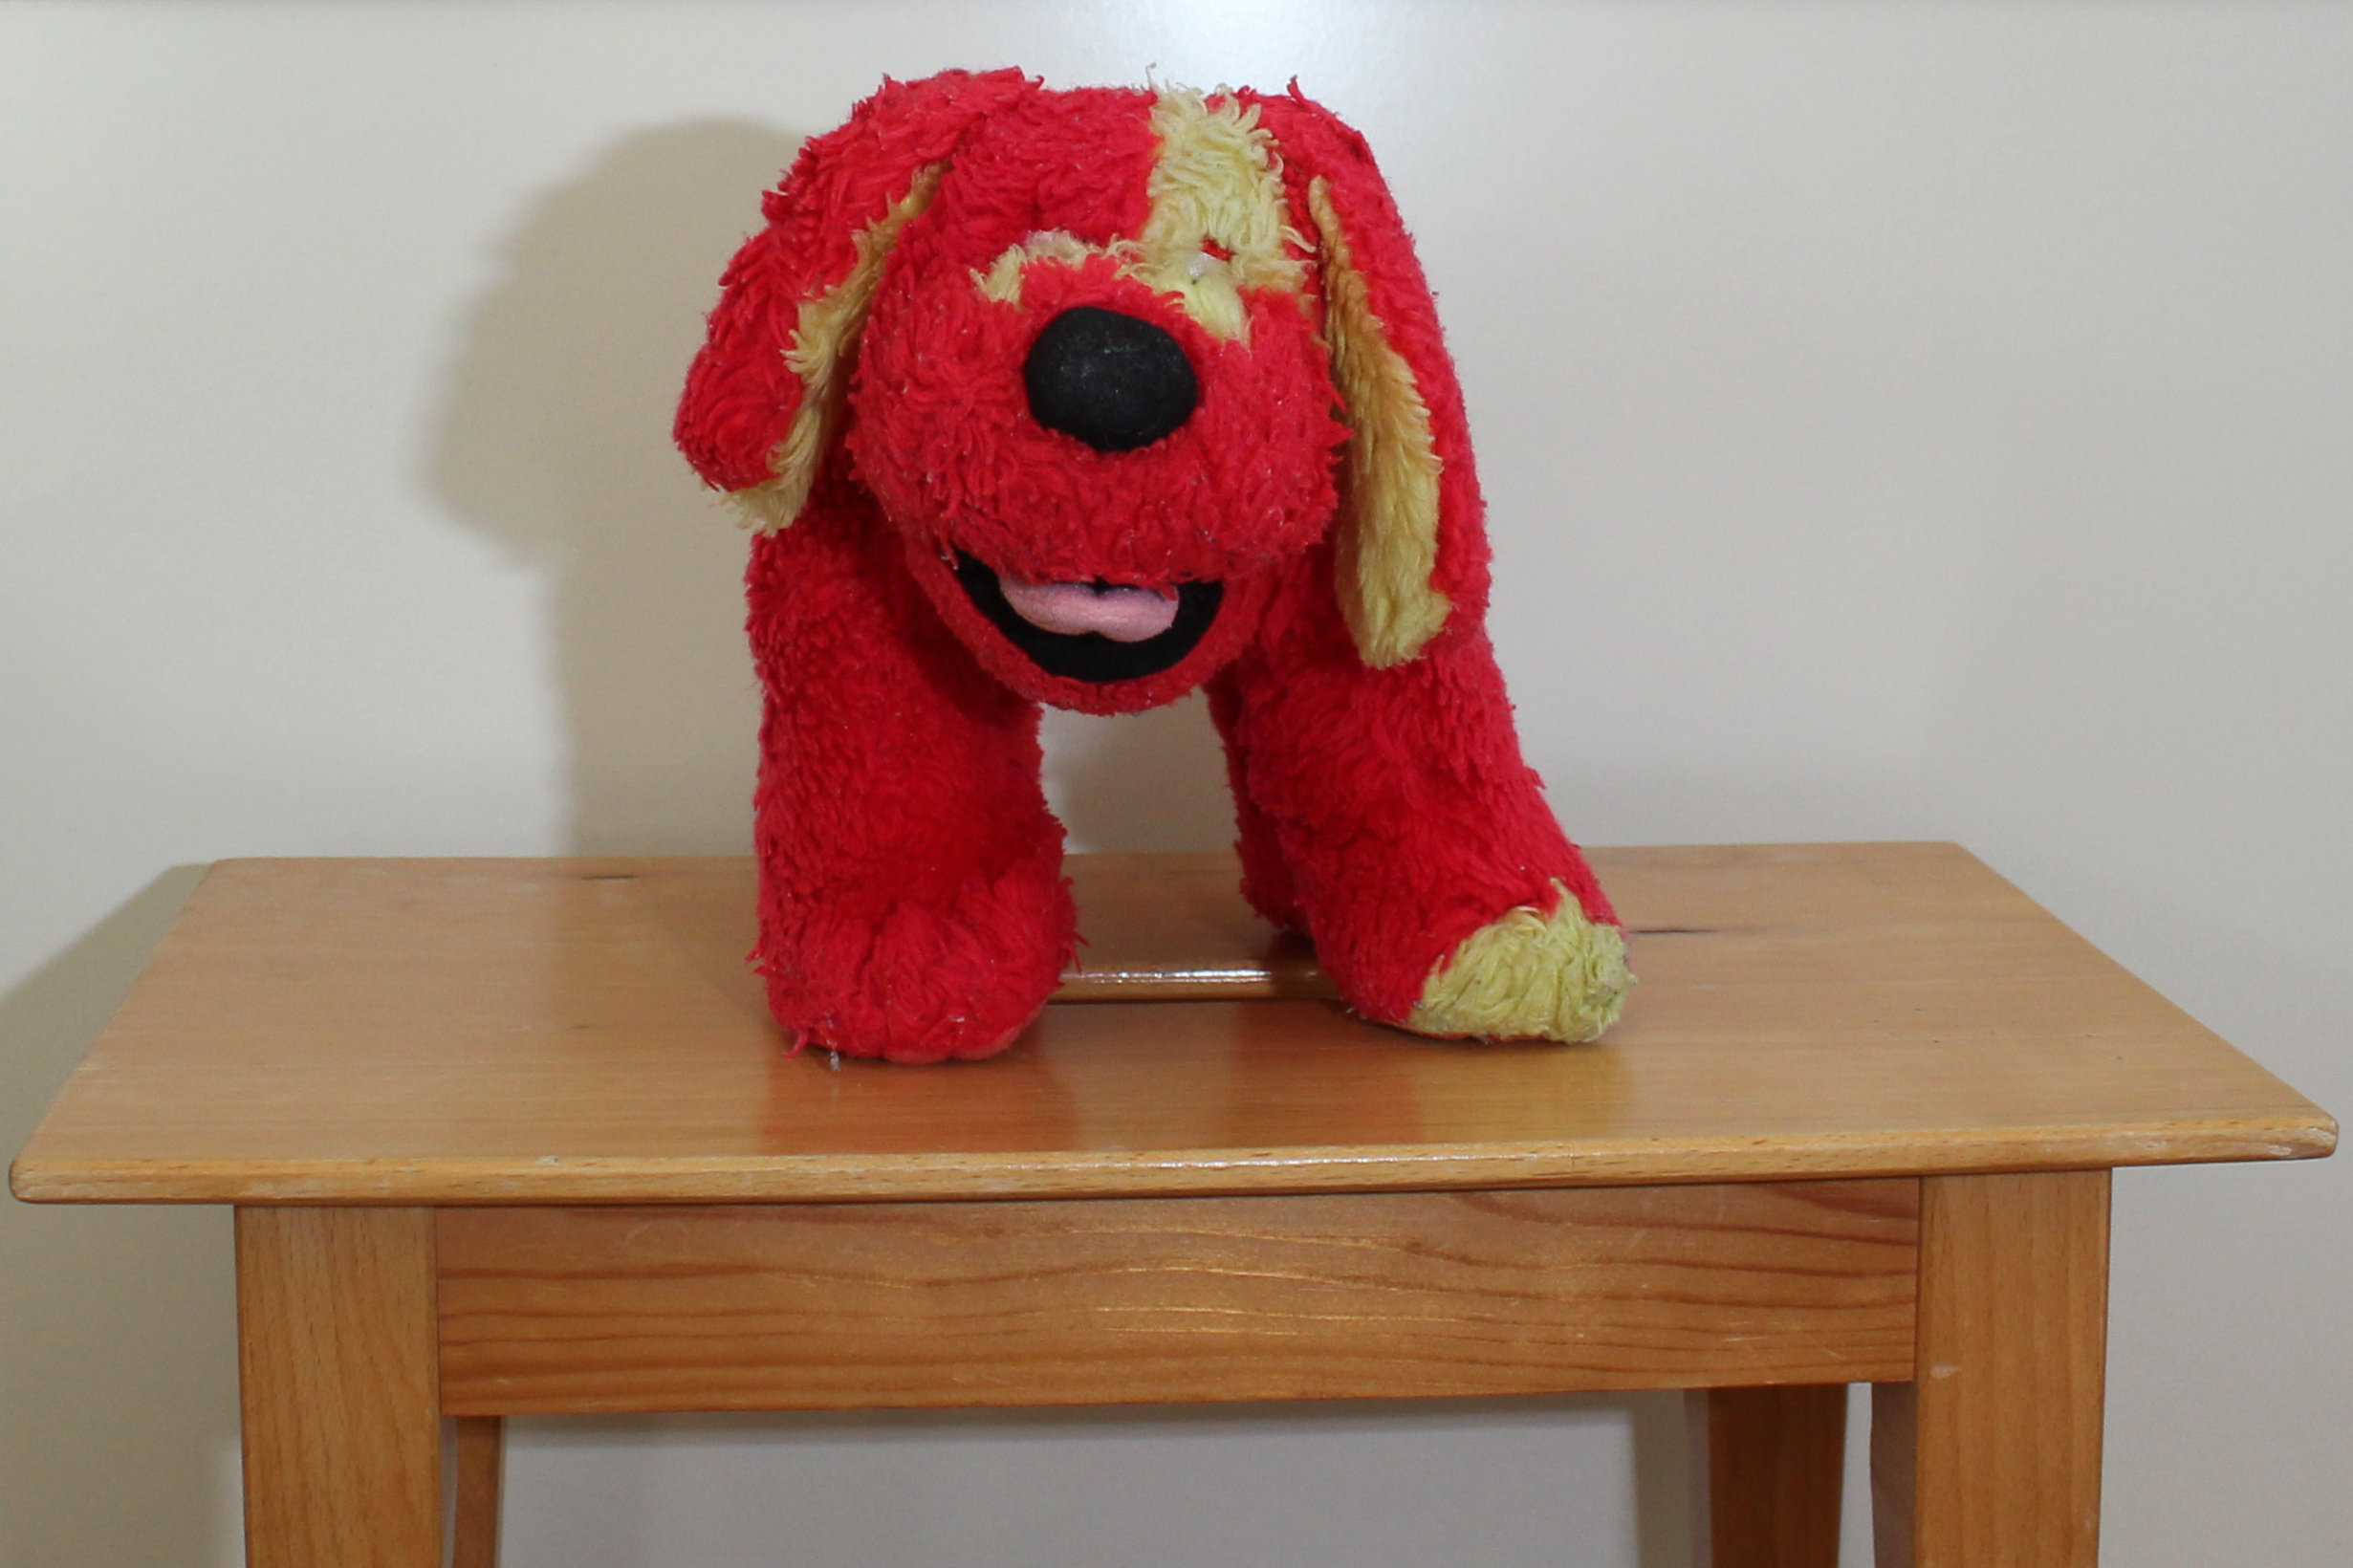
\includegraphics[width=1\textwidth]{blitz_seitlich.JPG}
    \caption{Beispielbild mit seitlichem Blitz.}
    \label{fig:seitlicher_blitzt}
\end{figure}

In der Abbildung \ref{fig:seitlicher_blitzt} ist zu sehen, dass durch die seitliche Platzierung des Blitzes 
auf der linken seite neben dem Motiv ein Schatten entsteht. Dieser Schatten ist unerwünscht und sollte
durch ein zentrales Blitzlicht vermieden werden.

\begin{figure}[H]
    \centering
    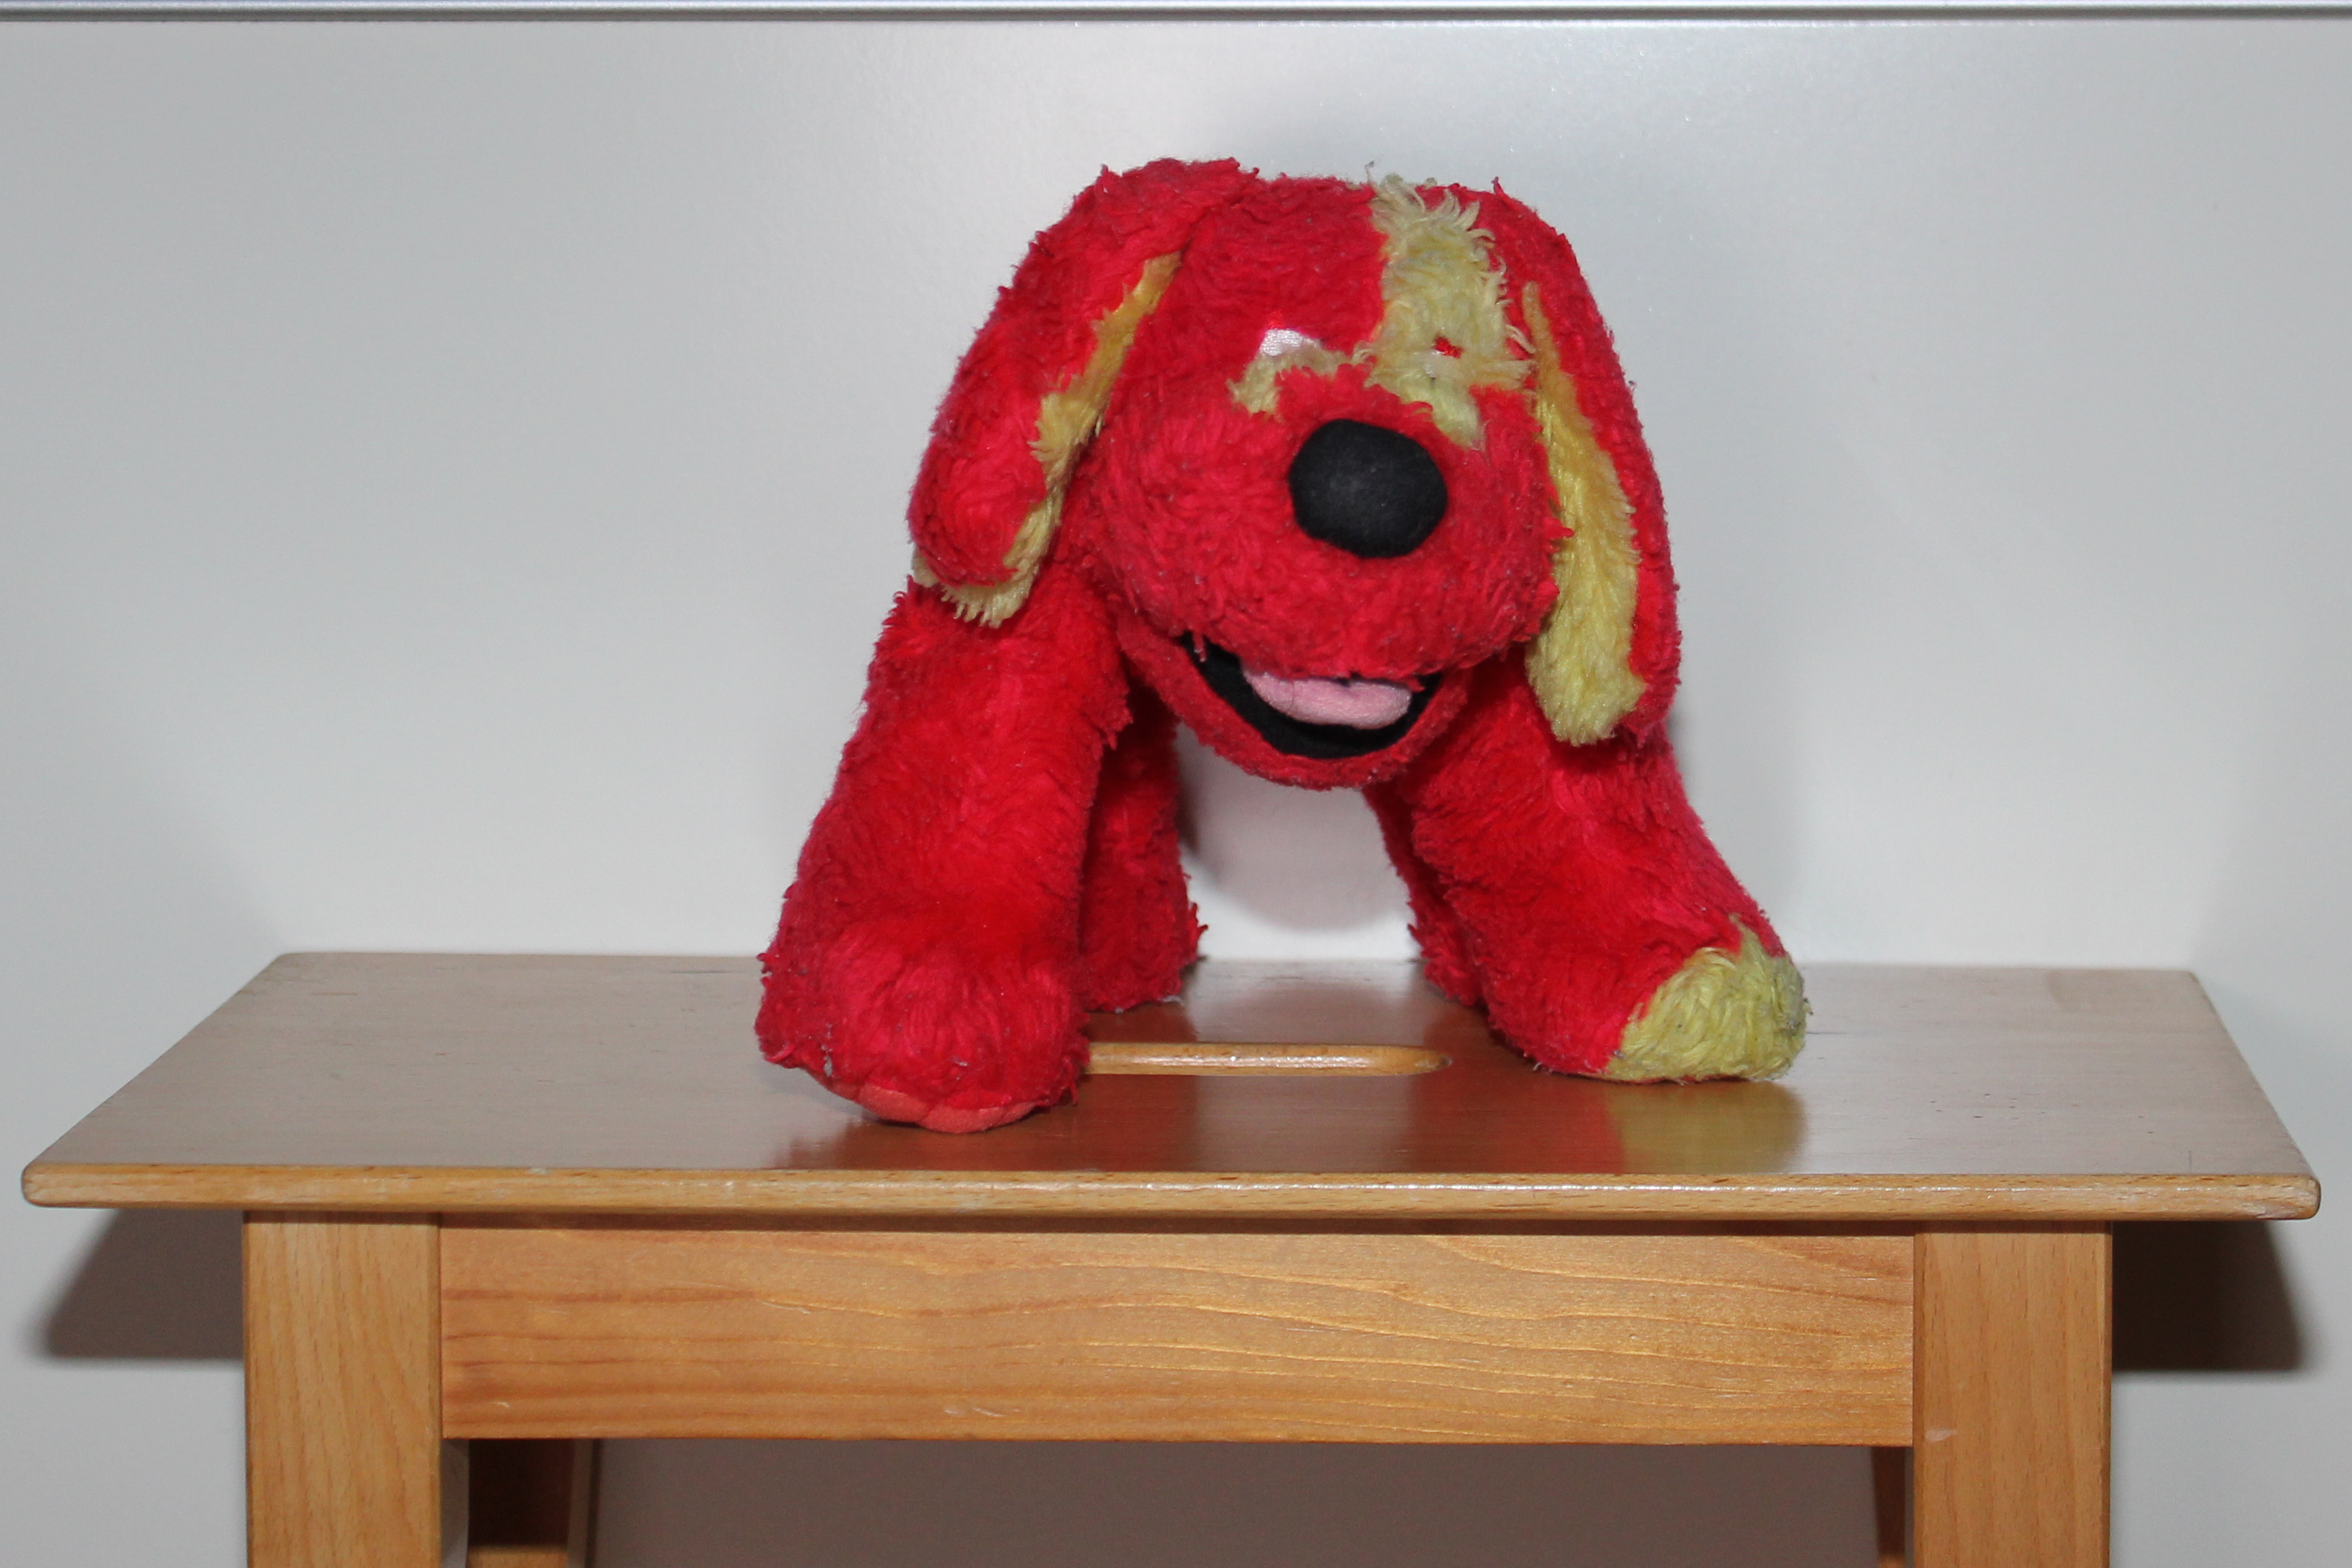
\includegraphics[width=1\textwidth]{blitz_vorne.JPG}
    \caption{Beispielbild mit zentralem Blitz.}
    \label{fig:zentraler_blitz}
\end{figure}

In der Abbildung \ref{fig:zentraler_blitz} ist zu sehen, dass durch die zentrale Platzierung des Blitzes,
das Bild deutlich besser ausgeleuchtet ist und keine seitlichen Schatten entstehen. 